%% Copyright (c) 2002, 2010 Sam Williams
%% Copyright (c) 2010 Richard M. Stallman
%% Copyright (c) 2014-2015 Posts & Telecommunications Press
%% Permission is granted to copy, distribute and/or modify this
%% document under the terms of the GNU Free Documentation License,
%% Version 1.3 or any later version published by the Free Software
%% Foundation; with no Invariant Sections, no Front-Cover Texts, and
%% no Back-Cover Texts. A copy of the license is included in the
%% file called ``gfdl.tex''.
\chapter{\ifdefined\eng
2001: A Hacker's Odyssey
\fi
\ifdefined\chs
黑客路漫漫
\fi}
\thispagestyle{empty}
\ifdefined\eng
The New York University computer-science department sits inside Warren Weaver Hall, a fortress-like building located two blocks east of Washington Square Park. Industrial-strength air-conditioning vents create a surrounding moat of hot air, discouraging loiterers and solicitors alike. Visitors who breach the moat encounter another formidable barrier, a security check-in counter immediately inside the building's single entryway.
\fi

\ifdefined\chs
纽约大学计算机学院坐落在沃伦·韦弗大楼(Warren Weaver Hall)之中,和著名的华盛顿广场公园相隔两个街区。大楼周围充斥着从空调压缩机里传出来的股股热浪,这阵热浪好似屏障一般,驱散着各路闲杂人等。倘若冲破这道屏障,面前还会出现另一道防线:一个安检处拦在了整座大楼的唯一一道入口前面。
\fi

\ifdefined\eng
Beyond the security checkpoint, the atmosphere relaxes somewhat. Still, numerous signs scattered throughout the first floor preach the dangers of unsecured doors and propped-open fire exits. Taken as a whole, the signs offer a reminder: even in the relatively tranquil confines of pre-September 11, 2001, New York, one can never be too careful or too suspicious.
\fi

\ifdefined\chs
走过安检口,气氛似乎缓和了些。可是,依旧能看到各处林立的警示牌指向消防出口。一路下来,可能会有这样的感受:哪怕是在2001年9月初的纽约这样一座现代化的都市之中,也要记得,小心驶得万年船。
\fi

\ifdefined\eng
The signs offer an interesting thematic counterpoint to the growing number of visitors gathering in the hall's interior atrium. A few look like NYU students. Most look like \ifdefined\vone shaggy-aired \fi\ifdefined\vtwo shaggy-haired \fi concert-goers milling outside a music hall in anticipation of the main act. For one brief morning, the masses have taken over Warren Weaver Hall, leaving the nearby security attendant with nothing better to do but watch Ricki Lake on TV and shrug her shoulders toward the nearby auditorium whenever visitors ask about ``the speech.''
\fi

\ifdefined\chs
当继续向前,走到中央大厅的时候,这份谨慎的感受却被一群人冲破了。他们之中,有些看起来像是纽约大学的学生。大部分则蓬着头,好似等待着一场盛大的音乐会。在这短暂的上午,这群人占据了沃伦·韦弗大楼。这下子,安检人员反倒闲下来了。他们斜躺坐在椅子上,看着电视剧。要是哪位访客,问起``演讲''的事,这位保安就会连话也懒得说一句,干脆冲着旁边的大礼堂一耸肩,然后继续看他的电视剧。
\fi

\ifdefined\eng
%% v1 v1 very small
Once inside the auditorium, a visitor finds the person who has forced this temporary shutdown of building security procedures. The person is Richard M. Stallman, founder of the GNU Project, original president of the Free Software Foundation, winner of the 1990 MacArthur Fellowship, winner of the Association of Computing Machinery's Grace Murray Hopper Award (also in 1990), corecipient of the Takeda Foundation's 2001 Takeda Award\ifdefined\vtwo \ for Social/Economic Betterment\fi, and former AI Lab hacker. As announced over a host of hacker-related web sites, including the GNU Project's own \url{http://www.gnu.org} site, Stallman is in Manhattan, his former hometown, to deliver a much anticipated speech in rebuttal to the Microsoft Corporation's recent campaign against the GNU General Public License.
\fi

\ifdefined\chs
%% TODO
有如此神通,能让保安放半天假的这位演讲者,此时正坐在大礼堂中。他就是理查德·M·斯托曼:GNU工程的创始人,自由软件基金会的第一任主席,1990年麦克阿瑟奖(MacArthur Fellowship)获得者,同年美国计算机协会(Association of Computing Machinery)格雷斯·莫瑞·霍普奖(Grace Murray Hopper Award)获得者,2001年日本武田基金会(Takeda Foundation)的武田奖(Takeda Award)共同获得者。当然,他也是人们熟悉的那位麻省理工学院人工智能实验室的黑客。前阵子黑客相关的网站上,包括GNU工程的官方网站上(\url{http://www.gnu.org}),都刊载了一条新闻:理查德·M·斯托曼将在他的家乡纽约曼哈顿发表演讲,回应微软在前些时候关于GNU通用公共许可证(GNU General Public License)的抨击。
\fi

\ifdefined\eng
%% v1 v2 big
\ifdefined\vone
The subject of Stallman's speech is the history and future of the free software movement. The location is significant. Less than a month before, Microsoft senior vice president Craig Mundie appeared at the nearby NYU Stern School of Business, delivering a speech blasting the General Public License, or GPL, a legal device originally conceived by Stallman 16 years before. Built to counteract the growing wave of software secrecy overtaking the computer industry-a wave first noticed by Stallman during his 1980 troubles with the Xerox laser printer-the GPL has evolved into a central tool of the free software community. In simplest terms, the GPL locks software programs into a form of communal ownership-what today's legal scholars now call the ``digital commons''-through the legal weight of copyright. Once locked, programs remain unremovable. Derivative versions must carry the same copyright protection-even derivative versions that bear only a small snippet of the original source code. For this reason, some within the software industry have taken to calling the GPL a "viral" license, because it spreads itself to every software program it touches.\endnote{Actually, the GPL's powers are not quite that potent. According to section 10 of the GNU General Public License, Version 2 (1991), the viral nature of the license depends heavily on the Free Software Foundation's willingness to view a program as a derivative work, not to mention the existing license the GPL would replace.

If you wish to incorporate parts of the Program into other free programs whose distribution conditions are different, write to the author to ask for permission. For software that is copyrighted by the Free Software Foundation, write to the Free Software Foundation; we sometimes make exceptions for this. Our decision will be guided by the two goals of preserving the free status of all derivatives of our free software and of promoting the sharing and reuse of software generally.

``To compare something to a virus is very harsh,'' says Stallman. ``A spider plant is a more accurate comparison; it goes to another place if you actively take a cutting.''

For more information on the GNU General Public License, visit \url{http://www.gnu.org/copyleft/gpl.html}.}
\fi
\ifdefined\vtwo
The subject of Stallman's speech is the history and future of the free software movement. The location is significant. Less than a month before, Microsoft senior vice president Craig Mundie appeared at the nearby NYU Stern School of Business, delivering a speech blasting the GNU General Public License, or GNU GPL, a legal device originally conceived by Stallman 16 years before. Built to counteract the growing wave of software secrecy overtaking the computer industry - a wave first noticed by Stallman during his 1980 troubles with the Xerox laser printer - the GPL has evolved into a central tool of the free software community. In simplest terms, the GPL establishes a form of communal ownership - what today's legal scholars now call the ``digital commons'' - through the legal weight of copyright. The GPL makes this irrevocable; once an author gives code to the community in this way, that code can't be made proprietary by anyone else. Derivative versions must carry the same copyright license, if they use a substantial amount of the original source code. For this reason, critics of the GPL have taken to calling it a ``viral'' license, suggesting inaccurately that it spreads itself to every software program it touches.\endnote{Actually, the GPL's powers are not quite that potent: just putting your code in the same computer with a GPL-covered program does not put your code under the GPL.

``To compare something to a virus is very harsh,'' says Stallman. ``A spider plant is a more accurate comparison; it goes to another place if you actively take a cutting.''

For more information on the GNU General Public License, visit \url{http://www.gnu.org/copyleft/gpl.html}.}
\fi
\fi

\ifdefined\chs
%% TODO
斯托曼演讲的主题,是关于自由软件运动的历史和未来。这次演讲的地点尤为重要。不到一个月前,微软的副总裁克雷格·蒙迪(Craig Mundie)就是出现在纽约大学斯特恩商学院(Stern School of Business),抨击GNU通用公共许可证——简称GPL。GPL是斯托曼16年前想出来的法律武器,用来对抗工业界中越来越盛行的专有软件。1980年,斯托曼经历了那次施乐打印机事件之后,预感到了软件专有化的潮流逐渐到来。为了抗衡这潮流,斯托曼提出了自由软件的概念:用户可以自由地使用、学习、修改和再发布软件。如今,GPL已经俨然成为了自由软件社区的核心工具。简单来说,GPL是一个软件使用许可证,它利用版权法,将自由软件锁定在公众可以自由使用和修改的领域。一旦锁定,这个软件就不会再被专有化。不仅仅是这个软件本身被锁定为自由软件,这个软件的任何衍生品也会成为自由软件。也就是说,倘若某个软件以GPL形式授权发布,这个软件以及任何它的衍生品,都可以被用户自由使用和修改。所谓一个软件的衍生品,也就是任何使用了该软件的代码的作品。哪怕一个软件仅仅使用了某个GPL授权软件的一小部分代码,这个软件也将被要求以自由软件形式发布。恰恰是这个原因,软件业的很多人把GPL称为病毒式许可证,因为它像病毒一样,``感染''所有它触及到的程序\endnote{事实上,GPL的没有这么夸张的``威力''。把程序与另一个GPL许可证的程序放在同一台计算机上运行并不会把程序也变成自由软件。

斯托曼说:``把一个东西说成是病毒是一种很粗暴的类比,也许把GPL比成是吊兰还稍微贴切一些,如果你把它切下来放到别处,它会继续生长。''

要了解GNU通用公共许可证的更多信息,请访问:\url{http://www.gnu.org/copyleft/gpl.html}
}。

\fi

\ifdefined\eng
%% v1 v2 small
\ifdefined\vone
In an information economy increasingly dependent on software and increasingly beholden to software standards, the GPL has become the proverbial ``big stick.'' Even companies that once laughed it off as software socialism have come around to recognize the benefits. Linux, the Unix-like kernel developed by Finnish college student Linus Torvalds in 1991, is licensed under the GPL, as are many of the world's most popular programming tools: GNU Emacs, the GNU Debugger, the GNU C Compiler, etc. Together, these tools form the components of a free software operating system developed, nurtured, and owned by the worldwide hacker community. Instead of viewing this community as a threat, high-tech companies like IBM, Hewlett Packard, and Sun Microsystems have come to rely upon it, selling software applications and services built to ride atop the ever-growing free software infrastructure.
\fi
\ifdefined\vtwo
In an information economy increasingly dependent on software and increasingly beholden to software standards, the GPL has become the proverbial ``big stick.'' Even companies that once derided it as ``software socialism'' have come around to recognize the benefits. Linux, the kernel developed by Finnish college student Linus Torvalds in 1991, is licensed under the GPL, as are most parts of the GNU system: GNU Emacs, the GNU Debugger, the GNU C Compiler, etc. Together, these tools form the components of the free software GNU/Linux operating system, developed, nurtured, and owned by the worldwide hacker community. Instead of viewing this community as a threat, high-tech companies like IBM, Hewlett Packard, and Sun Microsystems have come to rely upon it, selling software applications and services built to ride atop the ever-growing free software infrastructure.\endnote{Although these applications run on GNU/Linux, it does not follow that they are themselves free software.  On the contrary, most of them applications are proprietary software, and respect your freedom no more than Windows does.  They may contribute to the success of GNU/Linux, but they don't contribute to the goal of freedom for which it exists.}
\fi
\fi

\ifdefined\chs
%% TODO
随着信息产业的发展,全球越来越依赖软件和软件标准。在这样的环境下,谁都无法忽视GPL。哪怕曾经嘲笑过GPL的公司,也不能再把它视为空中楼阁。因为越来越多的软件都是以GPL形式授权:Linux,一个最初由芬兰大学生林纳斯·托瓦兹(Linus Torvalds)于1991年开发出的类UNIX操作系统内核、GNU Emacs、GNU调试器、GNU编译器等都是以GPL授权的。这些工具在一起,形成了一个完整的自由操作系统。世界各地的黑客为这套操作系统贡献着代码。每个黑客也可以自由地拥有这样一套操作系统。如今,很多计算机公司都不再把这样一套自由操作系统视为威胁。相反,IBM、惠普、Sun等公司都依赖这个操作系统,并在这套系统之上开发和出售自己的软件产品。
\ifdefined\vtwo
%\endnote{仅管这些软件都在GNU/Linux上运行,但它们本身不一定是自由软件,相反的,他们中的大部分都是私有软件。跟Windows一样,这些私有软件同样不尊重你的自由。虽然它们对于GNU/Linux的成功起到了一定的推动作用,但它们对于自由软件运动中实现自由的目标并没有什么贡献。}
\fi
\fi

\ifdefined\eng
%% v1v2 m
\ifdefined\vone
They've also come to rely upon it as a strategic weapon in the hacker community's perennial war against Microsoft, the Redmond, Washington-based company that, for better or worse, has dominated the PC-software marketplace since the late 1980s. As owner of the popular Windows operating system, Microsoft stands to lose the most in an industry-wide shift to the GPL license. Almost every line of source code in the Windows colossus is protected by copyrights reaffirming the private nature of the underlying source code or, at the very least, reaffirming Microsoft's legal ability to treat it as such. From the Microsoft viewpoint, incorporating programs protected by the ``viral'' GPL into the Windows colossus would be the software equivalent of Superman downing a bottle of Kryptonite pills. Rival companies could suddenly copy, modify, and sell improved versions of Windows, rendering the company's indomitable position as the No. 1 provider of consumer-oriented software instantly vulnerable. Hence the company's growing concern over the GPL's rate of adoption. Hence the recent Mundie speech blasting the GPL and the " open source" approach to software development and sales. And hence Stallman's decision to deliver a public rebuttal to that speech on the same campus here today.
\fi
\ifdefined\vtwo
They've also come to rely upon it as a strategic weapon in the hacker community's perennial war against Microsoft, the Redmond, Washington-based company that has dominated the PC-software marketplace since the late 1980s. As owner of the popular Windows operating system, Microsoft stands to lose the most in an industry-wide shift to the GPL license. Each program in the Windows colossus is covered by copyrights and contracts (End User License Agreements, or EULAs) asserting the proprietary status of the executable, as well as the underlying source code that users can't get anyway. Incorporating code protected by the ``viral'' GPL into one of these programs is forbidden; to comply with the GPL's requirements, Microsoft would be legally required to make that whole program free software. Rival companies could then copy, modify, and sell improved versions of it, taking away the basis of Microsoft's lock over the users.
\fi
\fi

\ifdefined\chs
%% TODO
在黑客这个圈子里,这个操作系统也被当作战略武器,用来对抗微软公司。这个总部坐落于华盛顿州雷德蒙德市的软件公司,从20世纪80年代开始,已经俨然成了软件业的垄断巨头。作为Windows操作系统的拥有者,微软公司面对业界同行转向GPL许可证的事实,已经再也坐不住了。在Windows中,几乎每行代码都是专有的。至少按照法律条款看,它归微软所有。倘若有谁不慎在Windows中放入一点GPL授权的代码,整个Windows产品都会被``感染''为自由软件。在微软看来,这就好比把哪吒请进了龙宫,整个公司都得翻江倒海,它必须把整个操作系统的代码都以自由软件的形式发布。竞争对手就可以自由地复制、修改这个系统,并销售修改后的版本,这可能会瞬间颠覆微软公司龙头老大的地位。
\fi

\ifdefined\vtwo
\ifdefined\eng
%% v2 only
Hence the company's growing concern over the GPL's rate of adoption. Hence the recent Mundie speech blasting the GPL and the ``open source'' approach to software development and sales. (Microsoft does not even acknowledge the term ``free software,'' preferring to use its attacks to direct attention towards the apolitical ``open source'' camp described in \autoref{chapter:open source}, and away from the free software movement.) And hence Stallman's decision to deliver a public rebuttal to that speech on the same campus here today.
\fi

\ifdefined\chs
%% TODO
因此,微软极度关注GPL的普及情况。也正因如此,蒙迪才来纽约大学,抨击GPL以及``开源''软件的开发销售模式。(微软并不承认``自由软件''这个概念,而是习惯把矛头指向\autoref{chapter:open source}章节中即将谈到的``开源''阵营,回避自由软件运动的存在。)这才引得斯托曼也决定来纽约大学,在同一所校园内,回应蒙迪的抨击。
\fi
\fi

\ifdefined\eng
%% v1v2 medium
\ifdefined\vone
20 years is a long time in the software industry. Consider this: in 1980, when Richard Stallman was cursing the AI Lab's Xerox laser printer, Microsoft, the company modern hackers view as the most powerful force in the worldwide software industry, was still a privately held startup. IBM, the company hackers used to regard as the most powerful force in the worldwide software industry, had yet to to introduce its first personal computer, thereby igniting the current low-cost PC market. Many of the technologies we now take for granted-the World Wide Web, satellite television, 32-bit video-game consoles-didn't even exist. The same goes for many of the companies that now fill the upper echelons of the corporate establishment, companies like AOL, Sun Microsystems, Amazon.com, Compaq, and Dell. The list goes on and on.
\fi
\ifdefined\vtwo
20 years is a long time in the software industry. Consider this: in 1980, when Richard Stallman was cursing the AI Lab's Xerox laser printer, Microsoft, which dominates the worldwide software industry, was still a privately held startup. IBM, the company then regarded as the most powerful force in the computer hardware industry, had yet to introduce its first personal computer, thereby igniting the current low-cost PC market. Many of the technologies we now take for granted - the World Wide Web, satellite television, 32-bit video-game consoles - didn't even exist. The same goes for many of the companies that now fill the upper echelons of the corporate establishment, companies like AOL, Sun Microsystems, Amazon.com, Compaq, and Dell. The list goes on and on.
\fi
\fi

\ifdefined\chs
%% TODO
对软件业来说,二十年的时间可是个不短的年头。遥想二十多年前的1980年,斯托曼还在咒骂着人工智能实验室的施乐打印机;微软,这个被当今黑客视为全球软件业巨头的公司,还是个私人的创业小公司;而IBM,这个被当年的黑客视为全球计算机业巨头的公司,还没推出个人计算机;至于IBM的个人计算机推动了整个计算机业的发展,则是之后的事情了。而当今人们习以为常的很多技术,在那时都还没出现。包括WWW网络、卫星电视、32位终端游戏机等。如今的很多计算机巨头,在当时也一样还没建立。包括AOL、Sun、亚马逊、康柏、戴尔等。
\fi

\ifdefined\eng
%% v1v2 small
\ifdefined\vone
The fact that the high-technology marketplace has come so far in such little time is fuel for both sides of the GPL debate. GPL-proponents point to the short lifespan of most computer hardware platforms. Facing the risk of buying an obsolete product, consumers tend to flock to companies with the best long-term survival. As a result, the software marketplace has become a winner-take-all arena.\endnote{See  Shubha Ghosh, ``Revealing the Microsoft Windows Source Code,'' \textit{Gigalaw.com} (January, 2000), \url{http://www.gigalaw.com/articles/ghosh-2000-01-p1.html}} The current, privately owned software environment, GPL-proponents say, leads to monopoly abuse and stagnation. Strong companies suck all the oxygen out of the marketplace for rival competitors and innovative startups.
\fi
\ifdefined\vtwo
Among those who value progress above freedom, the fact that the high-technology marketplace has come so far in such little time is cited both for and against the GNU GPL.  Some argue in favor of the GPL, pointing to the short lifespan of most computer hardware platforms. Facing the risk of buying an obsolete product, consumers tend to flock to companies with the best long-term survival. As a result, the software marketplace has become a winner-take-all arena.\endnote{See  Shubha Ghosh, ``Revealing the Microsoft Windows Source Code,'' \textit{Gigalaw.com} (January, 2000), \url{http://www.gigalaw.com/}.} The proprietary software environment, they say, leads to monopoly abuse and stagnation. Strong companies suck all the oxygen out of the marketplace for rival competitors and innovative startups.
\fi
\fi

\ifdefined\chs
%% TODO
高科技产业在这短暂时间内迅速成长的过程中,则充斥着关于GPL的争论。GPL的支持者声称:由于计算机硬件平台的短暂寿命,为了避免买到过时产品,用户会倾向于购买大品牌的产品。由此带来的结果,造成了软件市场赢者通吃的局面\endnote{参考Shubha Ghosh于2000年1月在\textit{Gigalaw.com}上发表的文章Revealing the Microsoft Windows Source Code。\url{http://www.gigalaw.com/articles/ghosh-2000-01-p1.html}}。而如今,由于软件被认为是专有的,具有垄断地位的公司就会滥用它的权利,使得整个产业停滞不前。垄断企业会堵住所有去路,让竞争者无法生存,也让后起的创业公司无处立足。
\fi

\ifdefined\eng
%% v1v2 small
\ifdefined\vone GPL-opponents \fi\ifdefined\vtwo Others \fi argue just the opposite. Selling software is just as risky, if not more risky, than buying software, they say. Without the legal guarantees provided by \ifdefined\vone private \fi\ifdefined\vtwo proprietary \fi software licenses, not to mention the economic prospects of a privately owned ``killer app'' (i.e., a breakthrough technology that launches an entirely new market),\endnote{Killer apps don't have to be proprietary. \ifdefined\vone Witness, of course, the legendary Mosaic browser, a program whose copyright permits noncommercial derivatives with certain restrictions. \fi Still, I think the reader gets the point: the software marketplace is like the lottery. The bigger the potential payoff, the more people want to participate. For a good summary of the killer-app phenomenon, see Philip Ben-David, ``Whatever Happened to the `Killer App'?'', \textit{e-Commerce News} (December 7, 2000), \ifdefined\vone\url{http://www.ecommercetimes.com/perl/story/5893.html}\fi\ifdefined\vtwo\url{http://www.ecommercetimes.com/story/5893.html}\fi.} companies lose the incentive to participate. Once again, the market stagnates and innovation declines. As Mundie himself noted in his May 3 address on the same campus, the GPL's ``viral'' nature ``poses a threat'' to any company that relies on the uniqueness of its software as a competitive asset. Added Mundie:

\begin{quote}
It also fundamentally undermines the independent commercial software sector because it effectively makes it impossible to distribute software on a basis where recipients pay for the product rather than just the cost of distribution.\endnote{See Craig Mundie, ``The Commercial Software Model,'' senior vice president, Microsoft Corp., excerpted from an online transcript of Mundie's May 3, 2001, speech to the New York University Stern School of Business, \url{http://www.microsoft.com/presspass/exec/craig/05-03sharedsource.asp}.}
\end{quote}

\fi

\ifdefined\chs
%% TODO
GPL的反对者则恰恰相反。他们声称销售软件和购买软件一样,具有风险。倘若没有法律保证软件可以被专有化,人们将再也看不到杀手级应用的繁荣(所谓杀手级应用,即某种技术足以打开一片全新市场)\endnote{其实杀手级应用并不一定需要是专有化的。\ifdefined\vone 比如说,传奇的Mosaic浏览器,它的许可证就允许在一定的限制条件下对该程序进行非商业化的修改。\fi 读者应该这样来理解:软件市场就像买彩票一样,预期的收益越高,越多的人愿意参与其中。有关杀手级应用的现象,Philip Ben-David 2007年12月7日发表的文章《What Happened to the``Killer App''?》对此有清晰的阐述。\url{http://www.ecommercetimes.com/story/5893.html}},公司也将失去继续创新的动力。正如微软副总裁蒙迪于5月3日在纽约大学所说的,GPL的``病毒''特性为各大公司带来了威胁,威胁着它们赖以生存的软件产品。蒙迪道:

%% Patch Pending
\begin{quote}
它严重地威胁着独立的商业软件。出售软件不仅仅是要收回发行成本,还有更多的人力附加价值。而GPL则让这种买卖变成天方夜谭\endnote{参考微软资深副总裁克雷格·蒙迪的The Commercial Software Model一文,节选于他2001年5月3日在纽约大学斯特恩商学院所做的演讲。\url{http://www.microsoft.com/presspass/exec/craig/05-03sharedsource.asp}}。
\end{quote}

\fi

\ifdefined\eng
%% v1v2 small
\ifdefined\vone
The mutual success of GNU/ Linux, the amalgamated operating system built around the GPL-protected Linux kernel, and Windows over the last 10 years reveals the wisdom of both perspectives. Nevertheless, the battle for momentum is an important one in the software industry. Even powerful vendors such as Microsoft rely on the support of third-party software developers whose tools, programs, and computer games make an underlying software platform such as Windows more attractive to the mainstream consumer. Citing the rapid evolution of the technology marketplace over the last 20 years, not to mention his own company's admirable track record during that period, Mundie advised listeners to not get too carried away by the free software movement's recent momentum:
\fi
\ifdefined\vtwo
The mutual success of GNU/Linux and Windows over the last 10 years suggests that both sides on this question are sometimes right.  However, free software activists such as Stallman think this is a side issue. The real question, they say, isn't whether free or proprietary software will succeed more, it's which one is more ethical.

Nevertheless, the battle for momentum is an important one in the software industry. Even powerful vendors such as Microsoft rely on the support of third-party software developers whose tools, programs, and computer games make an underlying software platform such as Windows more attractive to the mainstream consumer. Citing the rapid evolution of the technology marketplace over the last 20 years, not to mention his own company's impressive track record during that period, Mundie advised listeners to not get too carried away by the free software movement's recent momentum:
\fi
\fi

\ifdefined\chs
%% TODO
在过去的十年中,无论是GNU/Linux还是Windows,都有了长足的进步,赢得了各自的成功。两者双赢的局面,似乎使得无论支持或反对GPL都有了足够的理由。但是,作为像斯托曼这样的自由软件活动家来说,成功并不是事情的关键。真正的问题并不是自由软件和专有软件哪个更为成功,而是哪个更道德。不管怎么说,这场自由软件与专有软件的战役在软件工业发展史上是一次重要的事件。哪怕像微软这样强大的企业,也需要第三方软件开发者。恰恰是他们开发的工具、程序、游戏,才使得Windows系统更加吸引用户。回顾近二十年软件业的发展,哪怕不提自家公司的成长,蒙迪依旧提醒他的听众,不要被自由软件运动的风潮吹昏头脑:
\fi

\ifdefined\eng
\begin{quote}
Two decades of experience have shown that an economic model that protects intellectual property and a business model that recoups research and development costs can create impressive economic benefits and distribute them very broadly.\endnote{\textit{Ibid.}}
\end{quote}
\fi

\ifdefined\chs
\begin{quote}
二十年的经验表明,保护知识产权的经济社会,配合降低研发成本的商业模式,可以极大地促进经济发展和财富分配\endnote{\textit{同上}}。
\end{quote}

\fi

\ifdefined\eng
Such admonitions serve as the backdrop for Stallman's speech today. Less than a month after their utterance, Stallman stands with his back to one of the chalk boards at the front of the room, edgy to begin.
\fi

\ifdefined\chs
这段来自蒙迪的警告,成了斯托曼今日演讲的背景。现在,距离蒙迪演讲后不到一个月,斯托曼就站在演讲礼堂前方,背对着黑板,摩拳擦掌,迫不及待地准备发表他的演说了。
\fi

\ifdefined\eng
If the last two decades have brought dramatic changes to the software marketplace, they have brought even more dramatic changes to Stallman himself. Gone is the skinny, clean-shaven hacker who once spent his entire days communing with his beloved PDP-10. In his place stands a heavy-set middle-aged man with long hair and rabbinical beard, a man who now spends the bulk of his time writing and answering email, haranguing fellow programmers, and giving speeches like the one today. Dressed in an aqua-colored T-shirt and brown polyester pants, Stallman looks like a desert hermit who just stepped out of a Salvation Army dressing room.
\fi

\ifdefined\chs
这二十年来,相比软件业翻天覆地的变化,斯托曼的改变则更加明显。当年他曾是那位精瘦、不留胡须的黑客,曾在那台PDP-10前,没日没夜地和它畅谈。而如今,在讲坛上的那位,已人近中年,发福、留发、蓄须。他会花大把时间回复邮件,在公众或程序员面前发表演说、组织演讲——正如今天这次一样。他今天穿着海蓝色的T恤和一条棕色的涤纶裤子,看起来好似刚刚踏出沙漠的隐士。
\fi

\ifdefined\eng
The crowd is filled with visitors who share Stallman's fashion and grooming tastes. Many come bearing laptop computers and cellular modems, all the better to record and transmit Stallman's words to a waiting Internet audience. The gender ratio is roughly 15 males to 1 female, and 1 of the 7 or 8 females in the room comes in bearing a stuffed penguin, the official Linux mascot, while another carries a stuffed teddy bear.
\fi

\ifdefined\chs
人群之中,则充斥着和斯托曼有着类似打扮的听众。很多人带着笔记本电脑和蜂窝调制解调器,以及各种录音录像设备,准备把斯托曼的演讲传上互联网,那里还有更多的听众等着他的言论。听众中,男女比例大约15∶1。大约每七八个女听众里,就有一位拿着企鹅的毛绒玩具,这是Linux的吉祥物,还有些女听众则抱着泰迪熊。
\fi

\ifdefined\vone
\ifdefined\eng
\begin{figure}[ht] \centering
  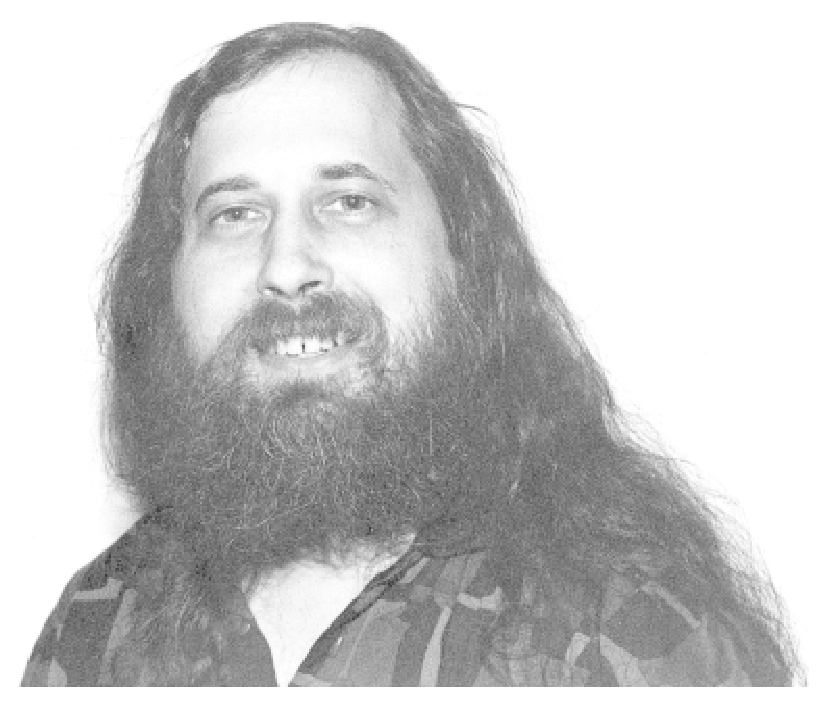
\includegraphics[width=\textwidth]{free_0201}
  \caption{Richard Stallman, circa 2000. "I decided I would develop a free software operating system or die trying . . . of old age of course." Photo courtesy of \url{http://www.stallman.org}.}
\end{figure}
\fi

\ifdefined\chs
\begin{figure}[ht] \centering
  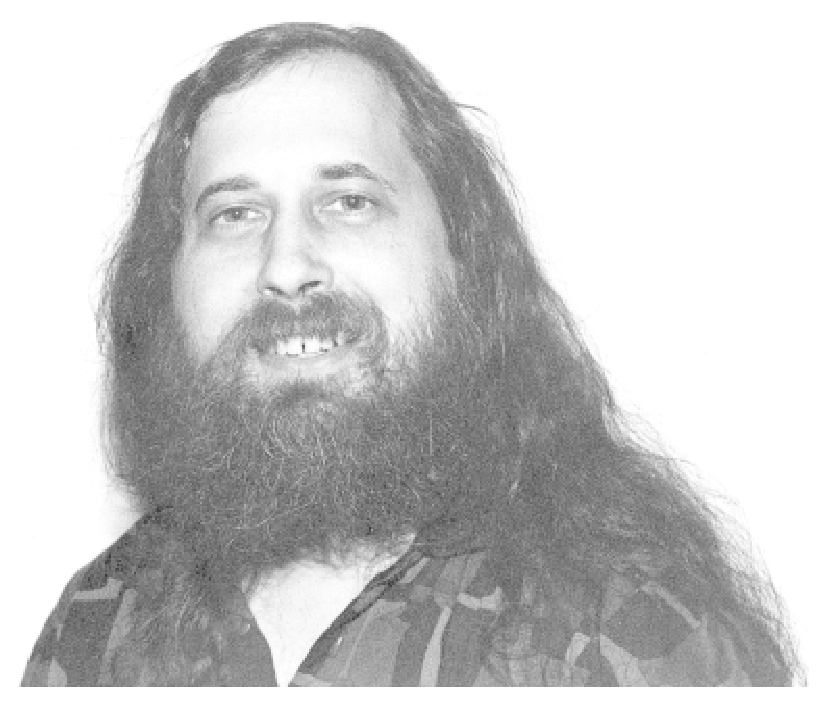
\includegraphics[width=\textwidth]{free_0201}
  \caption{图一\ 理查德·M·斯托曼,大约摄于2000年。``我决定要开发一套自由的操作系统,哪怕这要花费我一生的时间。''照片来自\url{http://www.stallman.org}。}
\end{figure}
\fi
\fi

\ifdefined\eng
%% v1v2 small
\ifdefined\vone
Agitated, Stallman leaves his post at the front of the room and takes a seat in a front-row chair, tapping a few commands into an already-opened laptop. For the next 10 minutes Stallman is oblivious to the growing number of students, professors, and fans circulating in front of him at the foot of the auditorium stage.
\fi
\ifdefined\vtwo
Agitated, Stallman leaves his post at the front of the room and takes a seat in a front-row chair, tapping commands into an already-opened laptop. For the next 10 minutes Stallman is oblivious to the growing number of students, professors, and fans circulating in front of him at the foot of the auditorium stage.
\fi
\fi

\ifdefined\chs
%% TODO
人潮涌动,斯托曼则离开了演讲台,坐在第一排的听众席上,把一直运行着的笔记本电脑拿出来,开始敲键盘。接下来的十分钟里,进来的学生、教授和粉丝逐渐走到他旁边,围观他工作,而斯托曼对此则完全不在意。
\fi

\ifdefined\eng
Before the speech can begin, the baroque rituals of academic formality must be observed. Stallman's appearance merits not one but two introductions. Mike Uretsky, codirector of the Stern School's Center for Advanced Technology, provides the first.
\fi

\ifdefined\chs
既然在大学演讲,学院派的规矩是少不了的。演讲嘉宾介绍则是重要一环。对斯托曼的介绍可谓阵容强大。纽约大学的两位教授分别为他做两段开场白。第一位,是来自纽约大学斯特恩商学院高新技术研究中心的主任,麦克·乌列茨基(Mike Uretsky)。
\fi

\ifdefined\eng
``The role of a university is to foster debate and to have interesting discussions,'' Uretsky says. ``This particular presentation, this seminar falls right into that mold. I find the discussion of open source particularly interesting.''
\fi

\ifdefined\chs
%% Patch Pending
``大学之地,争辩之所;争辩之处,兴趣所在。''乌列茨基说,``本次讲座,恰是秉承此道。个人愚见,所谓开源,甚是有趣。''
\fi

\ifdefined\eng
Before Uretsky can get another sentence out, Stallman is on his feet waving him down like a stranded motorist.
\fi

\ifdefined\chs
还没等乌列茨基把话说完,斯托曼就站起来挥着手喊道:
\fi

\ifdefined\eng
``I do free software,'' Stallman says to rising laughter. ``Open source is a different movement.''
\fi

\ifdefined\chs
``我是搞自由软件的,开源是另外一码事!''
\fi

\ifdefined\eng
The laughter gives way to applause. The room is stocked with Stallman partisans, people who know of his reputation for verbal exactitude, not to mention his much publicized 1998 falling out with the open source software proponents. Most have come to anticipate such outbursts the same way radio fans once waited for Jack Benny's trademark, ``Now cut that out!'' phrase during each radio program.
\fi

\ifdefined\chs
这一嗓子引来了一阵哄堂大笑。笑声褪去,掌声渐起。当下,听众中绝大多数都对斯托曼的这份咬文嚼字有所耳闻,更知道在1998年,他和开源阵营支持者的那次争论。斯托曼的这一行为,就如同整点新闻一般,早在大家意料之中。
\fi

\ifdefined\eng
Uretsky hastily finishes his introduction and cedes the stage to Edmond Schonberg, a professor in the NYU computer-science department. As a computer programmer and GNU Project contributor, Schonberg knows which linguistic land mines to avoid. He deftly summarizes Stallman's career from the perspective of a modern-day programmer.
\fi

\ifdefined\chs
乌列茨基草草结束介绍,走下讲堂。接下来对斯托曼做介绍的,是纽约大学计算机系的教授埃德蒙·舍恩伯格(Edmond Schonberg)。作为一个计算机程序员,又是GNU工程的贡献者,他很清楚该如何用词。他站在当代程序员的角度,扼要回顾了斯托曼的事业。
\fi

\ifdefined\eng
``Richard is the perfect example of somebody who, by acting locally, started thinking globally [about] problems concerning the unavailability of source code,'' says Schonberg. ``He has developed a coherent philosophy that has forced all of us to reexamine our ideas of how software is produced, of what intellectual property means, and of what the software community actually represents.''\ifdefined\vtwo\endnote{If this were to be said today, Stallman would object to the term ``intellectual property'' as carrying bias and confusion. See \url{http://www.gnu.org/philosophy/not-ipr.html}.}\fi
\fi

\ifdefined\chs
``放眼全球,脚踏实地,斯托曼是典范。他严肃地审视了软件源代码不对公众公开的事实,发展出了一套严密的逻辑体系。这套体系敦促着我们,让我们不得不重新思考如何开发软件,何谓知识产权,以及软件社区究竟是何物。''\ifdefined\vtwo\endnote{如果他今天再来发表这样的演讲,斯托曼一定会指出``知识产权''这个词所存在的认识上的偏差和可能造成的混淆。请参考:\url{http://www.gnu.org/philosophy/not-ipr.html}}\fi
\fi

\ifdefined\eng
Schonberg welcomes Stallman to more applause. Stallman takes a moment to shut off his laptop, rises out of his chair, and takes the stage.
\fi

\ifdefined\chs
舍恩伯格的致辞迎来了更多的掌声。斯托曼在掌声中,合上笔记本电脑,挪出身子,走上讲台。
\fi

\ifdefined\eng
At first, Stallman's address seems more Catskills comedy routine than political speech. ``I'd like to thank Microsoft for providing me the opportunity to be on this platform,'' Stallman wisecracks. ``For the past few weeks, I have felt like an author whose book was fortuitously banned somewhere.''
\fi

\ifdefined\chs
演讲开始,斯托曼的表现更像是个老练的喜剧演员,让人没法察觉这是一场严肃的政论讲座。``我首先要感谢微软公司给了我这样一次机会,来到贵校,畅抒己见,”斯托曼玩笑道,“过去几周里,我都觉得自己像个没落作家,自己的作品都无人问津。''
\fi

\ifdefined\eng
For the uninitiated, Stallman dives into a quick free software warm-up analogy. He likens a software program to a cooking recipe. Both provide useful step-by-step instructions on how to complete a desired task and can be easily modified if a user has special desires or circumstances. ``You don't have to follow a recipe exactly,'' Stallman notes. ``You can leave out some ingredients. Add some mushrooms, 'cause you like mushrooms. Put in less salt because your doctor said you should cut down on salt - whatever.''
\fi

\ifdefined\chs
为了照顾新人,斯托曼用一套类比简要介绍了自由软件。他把软件代码比作烹饪菜谱。二者都提供清晰的步骤,说明如何一步一步完成某个特定任务。同时,人们都可以很容易地按照自己的需求,对它们进行修改。``你不用按照菜谱的每一步严格执行操作,''斯托曼说,``你可以少放点调料。喜欢蘑菇,放些蘑菇;口味淡就少放盐;加点胡椒粉什么的。''
\fi

\ifdefined\eng
Most importantly, Stallman says, software programs and recipes are both easy to share. In giving a recipe to a dinner guest, a cook loses little more than time and the cost of the paper the recipe was written on. Software programs require even less, usually a few mouse-clicks and a modicum of electricity. In both instances, however, the person giving the information gains two things: increased friendship and the ability to borrow interesting recipes in return.
\fi

\ifdefined\chs
最重要的,斯托曼强调,软件和菜谱都很容易被分享。倘若有位客人来家里吃晚餐,那么把菜谱给他无非是花些时间,费点笔墨。复制软件则要求更少,只要轻点鼠标,费点电。而分享之后,起码有两份收获:增进了友谊;同时,下次需要帮忙的时候,对方也会有所回报。
\fi

\ifdefined\eng
``Imagine what it would be like if recipes were packaged inside black boxes,'' Stallman says, shifting gears. ``You couldn't see what ingredients they're using, let alone change them, and imagine if you made a copy for a friend. They would call you a pirate and try to put you in prison for years. That world would create tremendous outrage from all the people who are used to sharing recipes. But that is exactly what the world of proprietary software is like. A world in which common decency towards other people is prohibited or prevented.''
\fi

\ifdefined\chs
``想象一下,要是菜谱全被封锁在一个黑匣子里,那会如何?''斯托曼话峰一转,``你不知道他们用了什么调料,只有他们才能更改配方。你如果把菜谱抄出一份,送给朋友,他们就把你叫贼,把你关进牢房,长达数年。如果你早就习惯了把菜谱传来传去,这样的世界一定会让你觉得不可理喻。可这一切恰恰发生在专有软件的世界之中。在这个世界里,很平常的社交行为被严格禁止,或者被想方设法避免。''
\fi

\ifdefined\eng
With this introductory analogy out of the way, Stallman launches into a retelling of the Xerox laser-printer episode. Like the recipe analogy, the laser-printer story is a useful rhetorical device. With its parable-like structure, it dramatizes just how quickly things can change in the software world. Drawing listeners back to an era before Amazon.com one-click shopping, Microsoft Windows, and Oracle databases, it asks the listener to examine the notion of software ownership free of its current corporate logos.
\fi

\ifdefined\chs
类比过后,斯托曼又提起了施乐打印机事件。和烹饪菜谱的类比一样,打印机事件也是一个称手的工具。两者介绍完,听众就可以了解到如今的软件业究竟发生了多大改变。斯托曼的介绍把听众拉回了曾经那个年代,那时还没有亚马逊和它的一键支付;没有微软和它的Windows系统;没有甲骨文数据库。在这样的背景之下,听众有了很大的想象空间,可以不受当下这些所谓的大公司影响,重新审视所谓的软件所有权。
\fi

\ifdefined\eng
Stallman delivers the story with all the polish and practice of a local district attorney conducting a closing argument. When he gets to the part about the Carnegie Mellon professor refusing to lend him a copy of the printer source code, Stallman pauses.
\fi

\ifdefined\chs
讲起施乐打印机事件,斯托曼轻车熟路。他好似律师在做法庭最后陈词一般,字斟句酌。当说到卡耐基梅隆大学的那位计算机教授拒绝给他源代码的时候,斯托曼道:
\fi

\ifdefined\eng
``He had betrayed us,'' Stallman says. ``But he didn't just do it to us. Chances are he did it to you.''
\fi

\ifdefined\chs
``他背叛了我们,''斯托曼稍有停顿,接着说,``但他不止背叛了我们,更有可能背叛你!''
\fi

\ifdefined\eng
On the word ``you,'' Stallman points his index finger accusingly at an unsuspecting member of the audience. The targeted audience member's eyebrows flinch slightly, but Stallman's own eyes have moved on. Slowly and deliberately, Stallman picks out a second listener to nervous titters from the crowd. ``And I think, mostly likely, he did it to you, too,'' he says, pointing at an audience member three rows behind the first.
\fi

\ifdefined\chs
%% Patch Pending
``你''字一出,斯托曼就伸出食指,指向在座听众。听众之中,有人稍有皱眉。而斯托曼的目光则移到了前排,一位听众正在低头偷笑。``而且我觉得,他更有可能背叛你''斯托曼指着刚才偷笑的那位听众。
%% ``你''字一出,斯托曼就伸出食指,指向在座听众。听众之中,有人稍有皱眉。而斯托曼的目光,则移到了前排,一位听众正在低头偷笑。``而且我觉得,他更有可能背叛你。''斯托曼指着刚才偷笑的那位听众。
\fi

\ifdefined\eng
By the time Stallman has a third audience member picked out, the titters have given away to general laughter. The gesture seems a bit staged, because it is. Still, when it comes time to wrap up the Xerox laser-printer story, Stallman does so with a showman's flourish. ``He probably did it to most of the people here in this room -- except a few, maybe, who weren't born yet in 1980,'' Stallman says, drawing more laughs. ``[That's] because he had promised to refuse to cooperate with just about the entire population of the planet Earth.''
\fi

\ifdefined\chs
%% Patch Pending
这个临场的包袱,把一个人的窃笑变成了全场大笑。各种行为,好似舞台剧一般。笑声中,他总结道:``要想不被他背叛,你只能盼着晚点投胎''笑声又起,``因为这位教授承诺,拒绝和地球上大多数人合作。''
%%这个临场的包袱,把一个人的窃笑变成了全场大笑。各种行为,好似舞台剧一般。笑声中,他总结道:``要想不被他背叛,你只能盼着晚点投胎。''笑声又起,``因为这位教授承诺,拒绝和地球上大多数人合作。''
\fi

\ifdefined\eng
Stallman lets the comment sink in for a half-beat. ``He had signed a nondisclosure agreement,'' Stallman adds.
\fi

\ifdefined\chs
斯托曼一字一顿:``他签署了保密协议。''
\fi

\ifdefined\eng
Richard Matthew Stallman's rise from frustrated academic to political leader over the last 20 years speaks to many things. It speaks to Stallman's stubborn nature and prodigious will. It speaks to the clearly articulated vision and values of the free software movement Stallman helped build. It speaks to the high-quality software programs Stallman has built, programs that have cemented Stallman's reputation as a programming legend. It speaks to the growing momentum of the GPL, a legal innovation that many Stallman observers see as his most momentous accomplishment.
\fi

\ifdefined\chs
在这二十年来,理查德⋅马修⋅斯托曼,从当年一个不太得志的学者,成为了一呼百应的运动领袖。这一蜕变本身就饱含寓意。它诉说着斯托曼的顽强与固执,诉说着他的决心和毅力,更清晰地诠释了自由软件运动的价值观和远见。这之中,也当然包含了斯托曼编写的高质量代码,字里行间都凝结了斯托曼的心血,将他的经历铸成了计算机界的传奇。传奇之上,更能看到GPL不可遏制的蓬勃生命力。而作为法律界的一大创新,GPL已经被公认为斯托曼的重要成就。
\fi

\ifdefined\eng
Most importantly, it speaks to the changing nature of political power in a world increasingly beholden to computer technology and the software programs that power that technology.
\fi

\ifdefined\chs
当下,计算机和相关软件技术已成为整个世界的一大支柱。斯托曼的经历也更彰显了在如此背景之下,政权民意的风云变化。
\fi

\ifdefined\eng
Maybe that's why, even at a time when most high-technology stars are on the wane, Stallman's star has grown. Since launching the GNU Project in 1984,\endnote{The acronym GNU stands for ``GNU's not Unix.'' In another portion of the May 29, 2001, NYU speech, Stallman summed up the acronym's origin:

\begin{quote}
We hackers always look for a funny or naughty name for a program, because naming a program is half the fun of writing the program. We also had a tradition of recursive acronyms, to say that the program that you're writing is similar to some existing program\ldots I looked for a recursive acronym for Something Is Not UNIX. And I tried all 26 letters and discovered that none of them was a word. I decided to make it a contraction. That way I could have a three-letter acronym, for Something's Not UNIX. And I tried letters, and I came across the word ``GNU.'' That was it.

Although a fan of puns, Stallman recommends that software users pronounce the ``g'' at the beginning of the acronym (i.e., ``gah-new''). Not only does this avoid confusion with the word ``gnu,'' the name of the African antelope, Connochaetes gnou, it also avoids confusion with the adjective ``new.'' ``We've been working on it for 17 years now, so it is not exactly new any more,'' Stallman says.
\end{quote}

Source: author notes and online transcript of ``Free Software: Freedom and Cooperation,'' Richard Stallman's May 29, 2001, speech at New York University, \url{http://www.gnu.org/events/rms-nyu-2001-transcript.txt}.} Stallman has been at turns ignored, satirized, vilified, and attacked -- both from within and without the free software movement. Through it all, the GNU Project has managed to meet its milestones, albeit with a few notorious delays, and stay relevant in a software marketplace several orders of magnitude more complex than the one it entered 18 years ago. So too has the free software ideology, an ideology meticulously groomed by Stallman himself.
\fi

\ifdefined\chs
这一切的一切,也许恰恰能解释,为什么斯托曼发起的运动能如此长久不衰,而很多当年的名牌大厂,却早已风光不再的原因。遥想当年,1984年,斯托曼刚刚发起了GNU工程\endnote{GNU是``GNU's not Unix''的缩写。斯托曼在2001年5月29日纽约大学的演讲中,讲述了这个缩写的起源:

\begin{quote}
作为黑客,我们总是想给程序起一些有趣或古怪的名字,因为给程序起名字也是编写程序的乐趣中的一部分。我们也有一种使用递归缩写的传统喜好,用这样的方式表明我们所新写的程序与某个现有的程序具有一定的相似性……在为GNU工程起名字时,我试图寻找一个递归缩写来表达``Something Is Not UNIX''含义,我用26个字母去取代``Something'',但得到的结果都差强人意,看起来并不像是一个单词。于是,我决定把Is这个单词采用缩写的形式,这样我就可以得到一个三个字母缩写词,也就是说是``Something's Not UNIX''。我尝试了各个字母,最终决定选用``GNU''这个词。

GNU作为一个双关词,斯托曼建议软件用户在发音时,对第一个字母``g''进行发音(也就是说,把它读作``gah-new'')。一方面是为了避免与表示白尾角马这种非州羚羊的单词``gnu''发生混淆,另一方面也是避免与``新(new)''这个形容词发生混淆。``我们已经为GNU工程奋斗了17年,因此它也一点也不`新'了。''
\end{quote}

来源:作者的笔记,以及斯托曼2001年5月29日在纽约大学演讲的在线讲稿``Free Software: Freedom and Cooperation''。\url{http://www.gnu.org/events/rms-nyu-2001-transcript.txt}
}。面对这一项目,自由软件运动内外都充斥着对这个工程的无视、嘲讽,甚至攻击。一路走来,虽然GNU工程有过几次跳票延期,但在大多数时候还能按时交付,完成一个又一个发布计划。踏过了十八个寒暑,GNU工程也日渐成熟,在软件市场中赢得一席之地。而这近二十年来,自由软件的理想被斯托曼精心呵护,渐渐传遍大江南北。
\fi

\ifdefined\eng
To understand the reasons behind this currency, it helps to examine Richard Stallman both in his own words and in the words of the people who have collaborated and battled with him along the way. The Richard Stallman character sketch is not a complicated one. If any person exemplifies the old adage ``what you see is what you get,'' it's Stallman.
\fi

\ifdefined\chs
要想了解这潮流背后的缘由,就要兼听八方言论。这不仅包括斯托曼自己的评价,更要倾听和他在同一战壕里作战的战友们的叙述。其实,斯托曼的个性并不复杂,倘若坚信``所见即所得'',那么斯托曼这个人就不难被理解。
\fi

\ifdefined\eng
``I think if you want to understand Richard Stallman the human being, you really need to see all of the parts as a consistent whole,'' advises Eben Moglen, legal counsel to the Free Software Foundation and professor of law at Columbia University Law School. ``All those personal eccentricities that lots of people see as obstacles to getting to know Stallman really \ifdefined\vone are \fi\ifdefined\vtwo `are' \fi Stallman: Richard's strong sense of personal frustration, his enormous sense of principled ethical commitment, his inability to compromise, especially on issues he considers fundamental. These are all the very reasons Richard did what he did when he did.''
\fi

\ifdefined\chs
``想要了解斯托曼这个人,你必须要把各处细节联系起来,看成一个有机的整体''伊本⋅莫格林说道,他是自由软件基金会法律顾问,同时也是哥伦比亚大学法学院教授,``在斯托曼身上有着各种古怪脾气,这也许会把人拒之千里。而这份不同寻常,恰恰就构成了斯托曼这个活生生的人。他对挫败异常敏感,他对道德准则恪守不渝。他不肯妥协的个性,在关键问题上不肯让步的固执,这一切的总和,最终让我们看到了当今的斯托曼。''
\fi

\ifdefined\eng
Explaining how a journey that started with a laser printer would eventually lead to a sparring match with the world's richest corporation is no easy task. It requires a thoughtful examination of the forces that have made software ownership so important in today's society. It also requires a thoughtful examination of a man who, like many political leaders before him, understands the malleability of human memory. It requires an ability to interpret the myths and politically laden code words that have built up around Stallman over time. Finally, it requires an understanding of Stallman's genius as a programmer and his failures and successes in translating that genius to other pursuits.
\fi

\ifdefined\chs
一个简单的打印机事件变成了燎原之火,燃遍全球,足以和全球最富有的软件公司抗衡。要想回顾和解释这一切,并非易事。首先要了解软件所有权,以及它是如何走到当今的重要位置的;更要和人类健忘的本性做斗争;还要能从关于斯托曼的各种神话和攻击之中,看出本质。最后,还要能理解斯托曼在软件领域的过人天赋;以及他如何把这份天赋用到其他领域;还有在这一过程中的各种成败得失。
\fi

\ifdefined\eng
When it comes to offering his own summary of the journey, Stallman acknowledges the fusion of personality and principle observed by Moglen. ``Stubbornness is my strong suit,'' he says. ``Most people who attempt to do anything of any great difficulty eventually get discouraged and give up. I never gave up.''
\fi

\ifdefined\chs
当我请斯托曼做一番自我总结的时候,他也强调了莫格林提到的个性和原则:``坚强固执是我的本性。很多人在尝试做一些事,遇到了困难,就退缩放弃了。可我从不言弃。''
\fi

\ifdefined\eng
He also credits blind chance. Had it not been for that run-in over the Xerox laser printer, had it not been for the personal and political conflicts that closed out his career as an MIT employee, had it not been for a half dozen other timely factors, Stallman finds it very easy to picture his life following a different career path. That being said, Stallman gives thanks to the forces and circumstances that put him in the position to make a difference.
\fi

\ifdefined\chs
他也同样感激自己的运气。倘若当初没有那次打印机事件,没有其中的各种人事冲突,没有当年的各种机缘巧合,他也许不会放弃麻省理工学院的研究职位,不会重新抉择,选择一条与众不同的道路,并为之奋斗终身。是身边的各种因素,最终让斯托曼得以做出不同凡响的成绩。
\fi

\ifdefined\eng
``I had just the right skills,'' says Stallman, summing up his decision for launching the GNU Project to the audience. ``Nobody was there but me, so I felt like, `I'm elected. I have to work on this. If not me, who?'\hspace{0.01in}''
\fi

\ifdefined\chs
``我正好有合适的技能,''斯托曼回顾着当初发起GNU工程的决定,总结道,``除了我以外,没人在做这事。我就觉得`责任在身,我若不做,舍我其谁。'\hspace{0.01in}''
\fi

\theendnotes
\setcounter{endnote}{0}
